% ============================================================
% Materials and Methods section -- meant to be \input{} or \include{}'d
% from a main manuscript file, not compiled standalone. Same
% bibliography/style requirements as introduction.tex (see that file's
% header comment). Also requires \usepackage{url} (or hyperref, which
% loads it) for the \url{} dataset-availability links in Section 3.1, and
% \usepackage{graphicx} for the \includegraphics{} figures in Section 3.3
% (figures/Encoding.pdf, hand-authored by the user -- not script-generated,
% edit it directly if it needs to change), Section 3.4
% (figures/transfer_functions.pdf from
% figures/make_transfer_function_diagram.py -- rerun that script if its
% description changes, rather than hand-editing the PDF), and Section 3.6
% (figures/CSO.pdf, hand-authored by the user, showing the original CSO
% winner/loser flow; figures/cso_tf_selector_diagram.pdf from
% figures/make_cso_tf_selector_diagram.py, extending that same visual
% language -- rounded swarm boxes, yellow population labels, pale-blue
% process labels, orange flow arrows -- with the proposed method's
% per-particle transfer-function-selector decode step; rerun that script,
% not CSO.pdf, if the algorithm changes).
% The transfer-function plot's closed forms were derived from the real
% project code and cross-checked against it by Monte Carlo simulation
% (asserted in the script itself) before being plotted as smooth curves;
% this process surfaced that transfer.py::v_shaped's docstring ("flips
% the previous bit with probability V(x)") does not match its own
% measured behavior (flip probability is actually 1-V(x), peaking at
% x=0) -- flagged here for awareness, not silently resolved either way;
% verify against Hashemi et al.'s literal Eq. 6-7 before treating either
% the docstring or the code as authoritative.
%
% CITATION STATUS: every \cite{...} below resolves to a real, verified
% entry in references.bib (Little:2008, Naranjo:2016, Cheng:2015, and the
% 5 baseline source papers, all already used and verified elsewhere in
% this manuscript).
%
% DATA STATUS: all dataset statistics (sample sizes, subject counts,
% feature counts, class balance) were read directly from
% `src/data_loader.py` and a live run of `python -m src.data_loader`, not
% recalled from memory or from the source papers' own stated counts. Two
% discrepancies against externally-quoted figures were found and are
% documented in the note in Section \ref{sec:3.1}: the Oxford subject
% count (32, vs. the commonly quoted "31 subjects") and the UCI
% repository listing's structured "197 instances" metadata field (vs.
% 195, which matches both the actual distributed data file and that same
% listing's own descriptive prose) -- confirmed by fetching the live UCI
% page at https://archive.ics.uci.edu/dataset/174/parkinsons, not assumed.
%
% ENCODING STATUS (as of the latest revision): the 7 reproduced baselines
% decode the classifier segment multi-hot (`decode_bits`, equal-weight
% soft voting) via each runner's `classifier_encoding="multi_hot"`
% default, over a D+5-dimensional position (D feature dims + 5 classifier
% dims) binarized by each baseline's own fixed transfer function. The
% proposed method (plain CSO, Section~\ref{sec:3.6}) instead searches over
% a 5+D+5-dimensional position laid out as [selector(5) | features(D) |
% classifiers(5)]: a leading 5-dim transfer-function-selector segment
% decoded via argmax (Section \ref{sec:3.4}) into which of 5 candidate
% transfer functions binarizes THIS particle's own trailing D+5 segment --
% so, unlike the baselines, the proposed method has no single fixed
% transfer function at all.
% `decode_bits_top1` remains selectable per-call via
% `classifier_encoding="top1"` for a cheaper single-classifier run. This
% exact choice has flipped multiple times across the project's history --
% if asked to touch this file again, RE-CONFIRM the current defaults in
% `src/optimizers/base.py`, `src/optimizers/transfer.py`, and
% `src/experiments/run_comparison.py` before assuming this description is
% still accurate.
% ============================================================

\section{Materials and Methods}
\label{sec:3}

\subsection{Datasets and Study Population}
\label{sec:3.1}

Two public, retrospective, previously collected acoustic datasets are
used; no new data were collected for this study.

\textbf{Oxford Parkinson's Disease Voice Dataset} \cite{Little:2008},
publicly available from the UCI Machine Learning Repository
(\url{https://archive.ics.uci.edu/dataset/174/parkinsons},
\url{https://doi.org/10.24432/C59C74}), comprises 195 sustained phonation
(vowel /a/) recordings from 32 subjects, drawn from the \texttt{name}
field's subject code (\emph{not} the 31 patients reported in the
dataset's originating clinical study -- see the note below), of whom 147
recordings (75.4\%) are labeled
Parkinsonian and 48 (24.6\%) healthy control, i.e. class-imbalanced at the
recording level. Each recording is described by 22 acoustic features,
including fundamental-frequency perturbation measures (jitter variants),
amplitude perturbation measures (shimmer variants), harmonics-to-noise
ratio, and nonlinear dynamical measures (RPDE, DFA, spread1/2, D2, PPE).
Subjects contribute multiple recordings each (approximately six on
average), which is the reason subject-grouped cross-validation
(Section~\ref{sec:3.2}) is required rather than a plain
record-level split.

\emph{Note on dataset provenance discrepancies:} the UCI repository
listing for this dataset states, in its structured metadata field, 197
instances -- but the same page's own descriptive text states "195 voice
recording[s]", matching both the actual data file distributed at that
listing and the 195 figure used throughout this study; the 197 figure
appears to be an error in UCI's own metadata field, not a discrepancy in
this project's data handling. Separately, the dataset's own subject-id
field yields 32 distinct groups when parsed programmatically
(\texttt{src/data\_loader.py}), one more than the 31-subject figure
usually quoted from the originating clinical study and from the same UCI
listing's descriptive text. For both figures, this project reports the
value empirically observed in the data file actually used, and flags the
discrepancy rather than silently adopting the externally-quoted number.

\textbf{Naranjo Replicated Acoustic Features Dataset} \cite{Naranjo:2016},
publicly available from the UCI Machine Learning Repository
(\url{https://archive.ics.uci.edu/dataset/489/parkinson+dataset+with+replicated+acoustic+features},
\url{https://doi.org/10.24432/C5701F}), comprises 240 recordings from 80
subjects (40 Parkinsonian, 40 healthy control -- perfectly class-balanced
at the subject level), each subject
contributing exactly 3 repeated recordings. Each recording is described by
45 acoustic features (jitter, shimmer, and amplitude-perturbation
variants together with a gender covariate), extracted specifically to
support test-retest reliability analysis across repeated recordings of
the same speaker -- making subject-grouped evaluation especially
important for this dataset, since its very design guarantees near-identical
repeated measurements per subject. This dataset is also the smaller of
the two datasets used to validate the mHGS baseline reproduced in this
study \cite{Hashim:2023}.

\subsection{Data Preprocessing and Subject-Grouped Cross-Validation}
\label{sec:3.2}

No missing values are present in either dataset; features are used in
their raw scale, with per-fold standardization applied inside each
classifier's own pipeline (Section~\ref{sec:3.6}) rather than
globally, to avoid leaking validation-fold statistics into training.

Every fitness evaluation performed by every optimizer in this study --
the proposed method and all 7 reproduced baselines -- uses 5-fold
\texttt{StratifiedGroupKFold} cross-validation, grouped by subject
identifier and stratified by class label. This guarantees that all
recordings from a given subject fall entirely within a single fold, so no
classifier ever trains on one recording from a subject while being
validated on another recording from that same subject. This is not a
routine methodological detail: a systematic review of 69 voice-based PD
detection studies found that only eight employed a genuinely
subject-independent validation strategy, while roughly 70\% relied on
plain $k$-fold or fixed train/test splits without any subject-level
separation \cite{SedighMalekroodi:2025} -- which allows a classifier to
implicitly learn subject-specific vocal characteristics rather than
disease status, inflating reported accuracy in a way that does not
transfer to unseen individuals. Out-of-fold predictions from all 5 folds
are concatenated before any performance metric is computed, so every
reported score is computed over the entire dataset under a strict
train/validation separation, not averaged across fold-level scores.

\subsection{Joint Transfer-Function-, Feature-, and Classifier Optimization Encoding}
\label{sec:3.3}

Every optimizer in this study searches over a shared, particle-based
encoding: a continuous position vector of length $D + 5$, where $D$ is
the number of acoustic features in the dataset (22 for Oxford, 45 for
Naranjo). The first $D$ dimensions binarize, via each optimizer's own
transfer function, into a feature-selection mask over the $D$ acoustic
features. The last 5 dimensions correspond to five candidate base
classifiers, each with recent precedent as the wrapped classifier in its
own evolutionary/metaheuristic feature-selection study: support vector
machine (SVM, RBF kernel, calibrated via 3-fold Platt scaling for
probability estimates \cite{Platt:1999}; paired with PSO-based feature
selection for Alzheimer's disease diagnosis in \cite{Zhang:2025}), random
forest (RF, 100 trees; paired with an improved genetic algorithm for
feature selection in \cite{Ding:2025}), extreme gradient boosting
(XGBoost, 100 trees; paired with a multiobjective evolutionary algorithm
for biomarker feature selection in \cite{Panagiotopoulos:2023}),
$k$-nearest neighbors ($k$NN, $k=5$; paired with physics-inspired
metaheuristic feature selection in \cite{Priyadarshini:2023}), and
logistic regression (LogReg; paired with particle swarm optimization for
feature selection in chronic kidney disease diagnosis in
\cite{Mishra:2025}) -- chosen to span linear, instance-based, and both
bagged and boosted tree-ensemble decision boundaries, so the joint search
can in principle favor whichever inductive bias best matches each
dataset's feature space.

The last 5 dimensions are decoded the same way for every algorithm in this study: independent on/off switches, such that every classifier whose switch is on trains on the same selected feature subset, and the ensemble's out-of-fold prediction is the unweighted average of the active classifiers' predicted probabilities (equal-weight soft voting) -- letting a metaheuristic search directly over which base learners join a voting ensemble, rather than fixing the ensemble's membership in advance, mirrors the automatic classifier-subset selection used to build majority-voting ensembles for HIV-1 protease cleavage-site prediction in \cite{Palmal:2023}. Applying this multi-classifier ensemble decoding uniformly, rather than letting each baseline fall back to whatever single-classifier scheme its own binarization naturally produces (an argmax over the same 5 scores), keeps the comparison in Section~\ref{sec:4} isolated to each method's \emph{search} strategy: every algorithm is optimizing over, and evaluated on, the identical solution space, so that a performance difference cannot be attributed to one method being handed a weaker or stronger classifier-selection scheme than another. If a particle ever decodes to an empty feature mask or an empty classifier mask, one bit is force-activated uniformly at random to keep the candidate solution evaluable.

\begin{figure}[t]
  \centering
  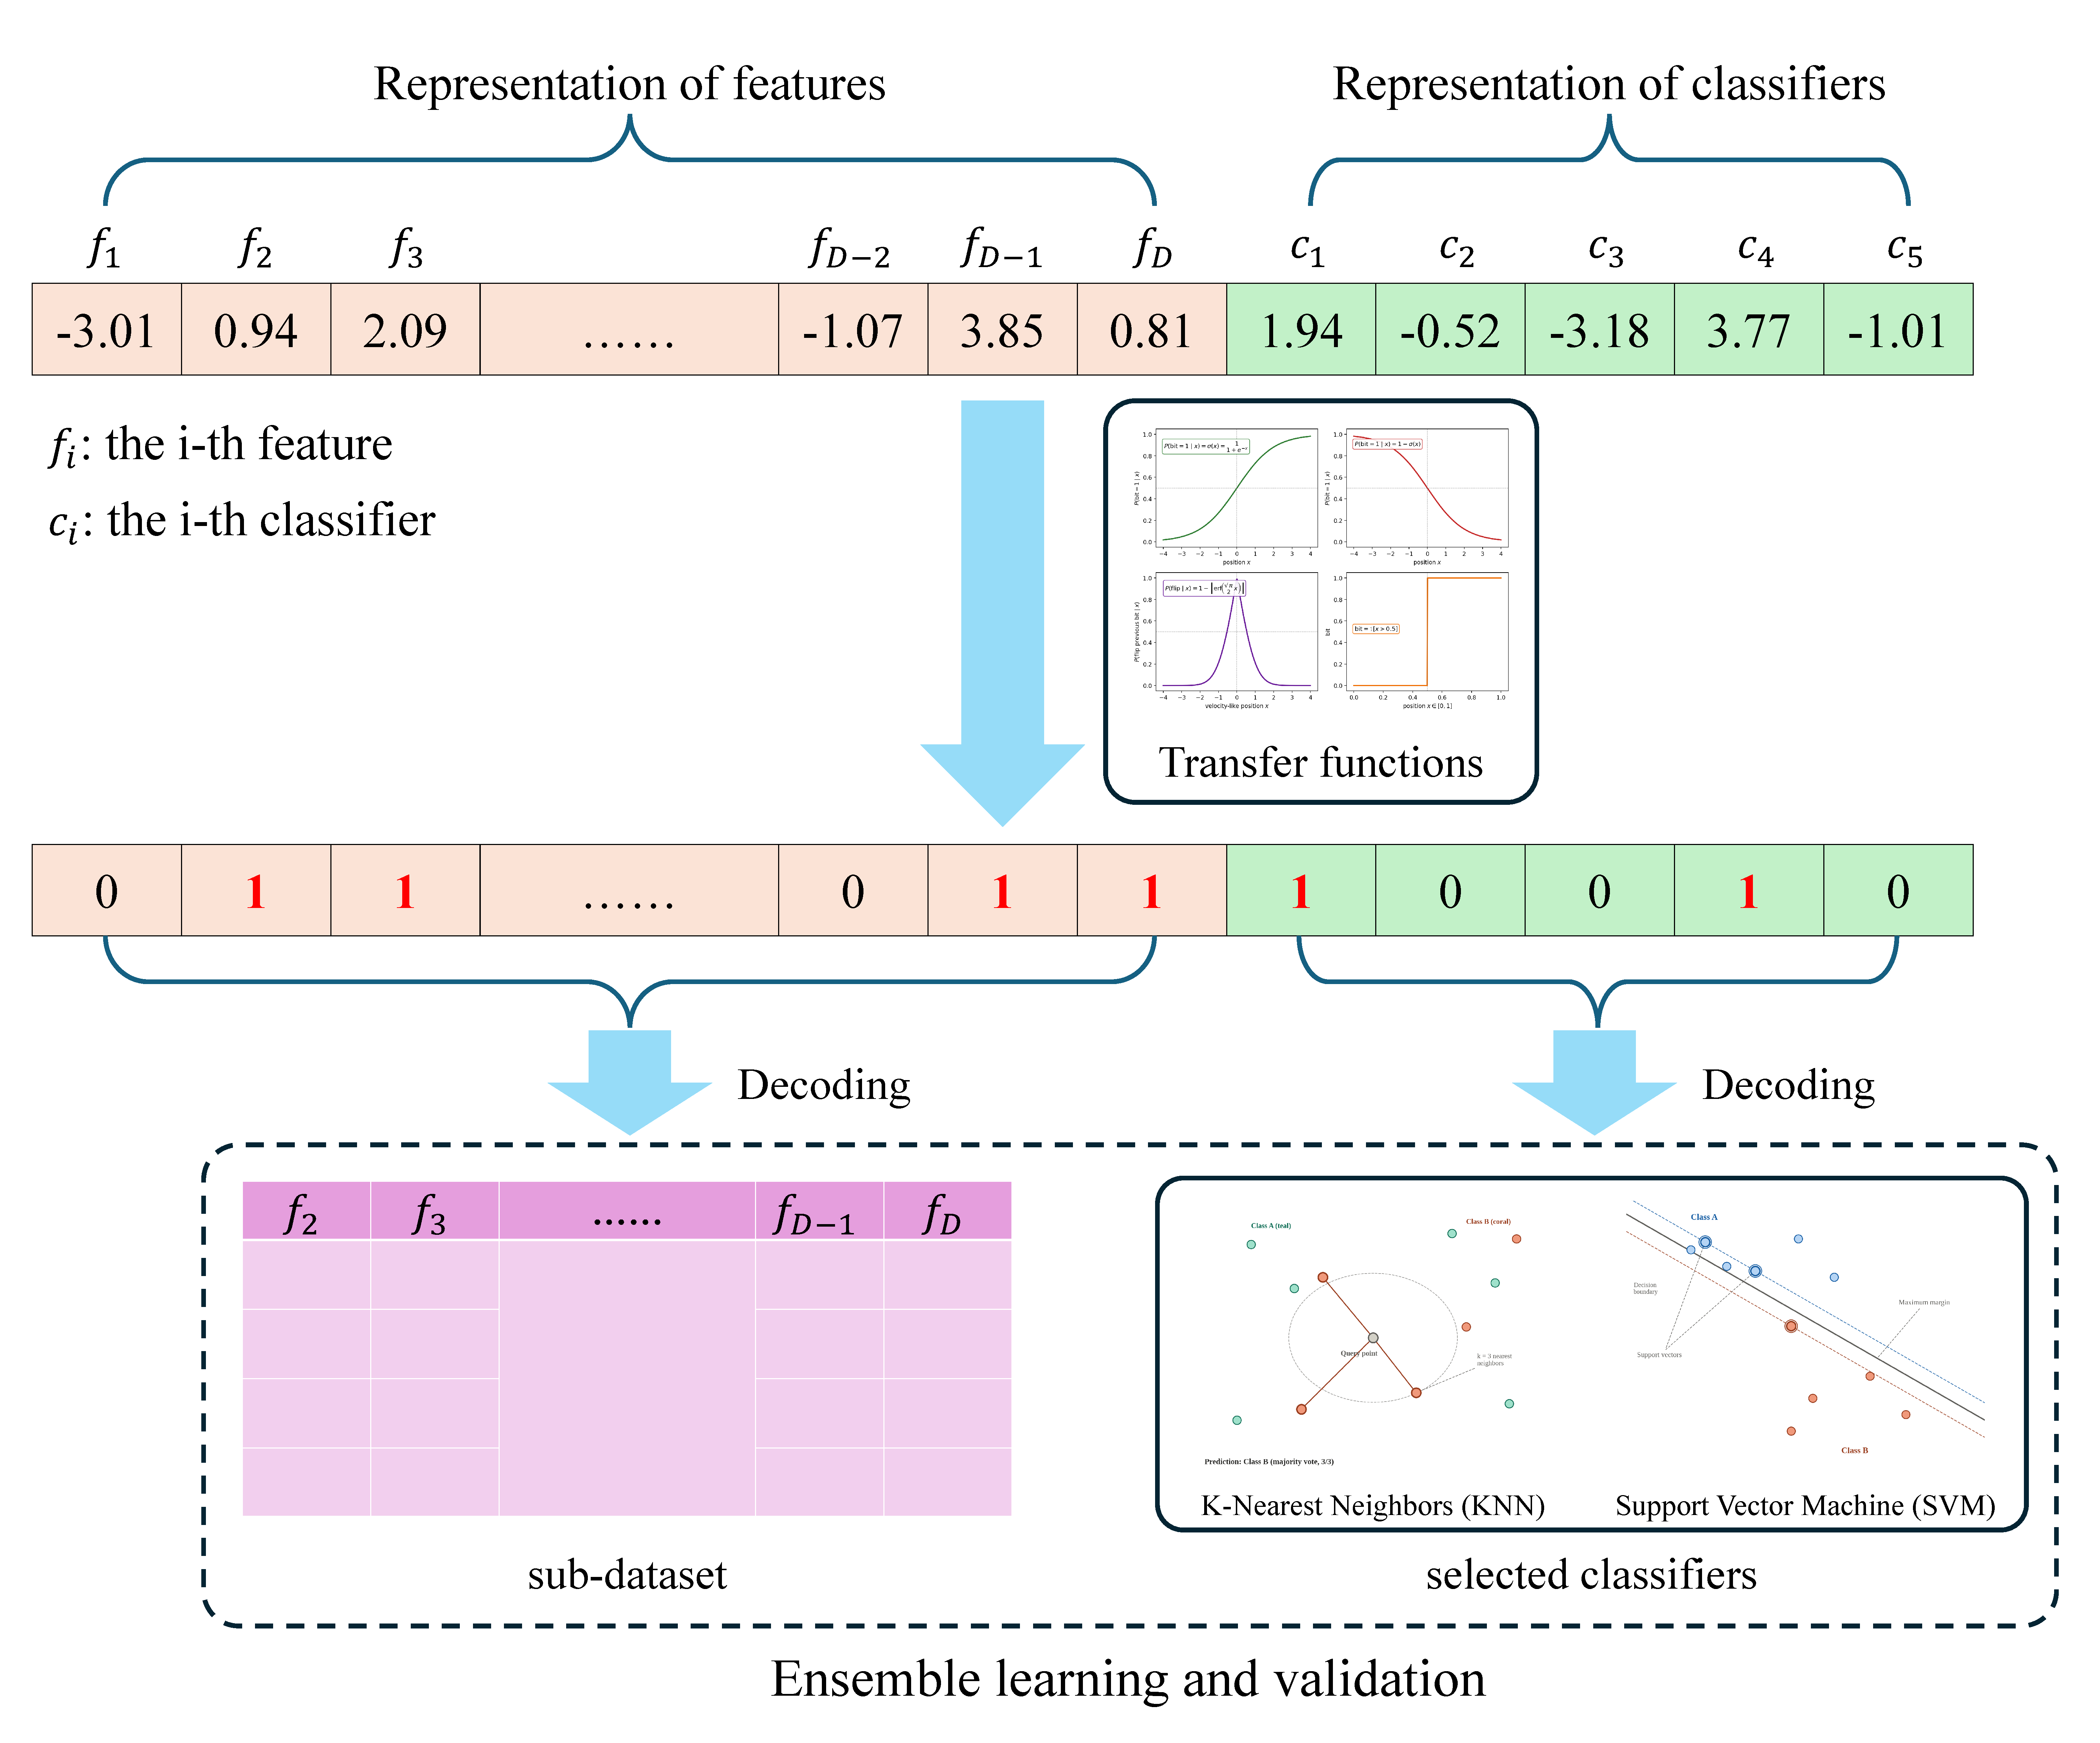
\includegraphics[width=\linewidth]{figures/Encoding.pdf}
  \caption{Worked example of the encoding and decoding pipeline shared by
    every algorithm in this study. A continuous particle position
    of length $D+5$ splits into $D$ feature scores ($f_1,\dots,f_D$) and 5
    classifier scores ($c_1,\dots,c_5$). Each segment passes through a
    transfer function (Figure~\ref{fig:transfer}) to produce a binary
    string; thresholded-off features/classifiers (0) are excluded and the
    remainder (1, highlighted) are decoded into a feature mask -- here
    selecting the sub-dataset restricted to columns $f_2, f_3, \ldots,
    f_{D-1}, f_D$ -- and a classifier mask -- here selecting SVM and
    $k$NN. Every classifier in the mask trains on the same feature subset
    and is combined by equal-weight soft voting before 5-fold
    subject-grouped cross-validation (Section~\ref{sec:3.5}).}
  \label{fig:encoding}
\end{figure}

Figure~\ref{fig:encoding} works through this pipeline end to end.

For the 7 reproduced baselines, this $D+5$-dimensional position is the
entire encoding, and it is binarized by whichever single transfer
function that baseline's own source paper specifies (Section
\ref{sec:3.4}). The proposed method (Section~\ref{sec:3.6}) prepends 5
further dimensions -- a transfer-function-selector segment
$t_1,\dots,t_5$, one score per candidate transfer function -- so each
particle's position has length $5+D+5$ and is laid out as
$[\,t_1,\dots,t_5 \mid f_1,\dots,f_D \mid c_1,\dots,c_5\,]$. The leading
selector segment is decoded the same way as the classifier segment's
top-1 alternative: an argmax over the raw continuous scores, with no
binarization step of its own, selecting exactly one of the 5 candidate
transfer functions described in Section~\ref{sec:3.4} -- deliberately
placed first so this choice is made independently of, and prior to, the
particle's trailing $D+5$ feature-and-classifier dimensions, whatever $D$
happens to be for the dataset at hand. That chosen function then
binarizes the trailing $D+5$ dimensions -- so, unlike every baseline, the
proposed method has no single transfer function fixed in advance: which
one applies is itself part of the search, and different particles in the
same generation may use different transfer functions.

\subsection{Transfer Functions for Binarization}
\label{sec:3.4}

The swarm- and population-based metaheuristics used in this study were,
in their original formulation, designed for continuous optimization: a
particle's position is a real-valued vector, and the search dynamics
(velocity updates, attraction toward better solutions, and so on) are
defined directly in terms of that continuous space. Joint
feature-and-classifier selection (Section~\ref{sec:3.3}) is inherently
discrete, however: each dimension of a solution must resolve to a binary
decision -- a given feature or classifier is either selected or it is
not. A \emph{transfer function} bridges this mismatch: it maps each
continuous position value to a probability (or, in the deterministic
case, applies a fixed threshold) that determines the corresponding bit,
so an optimizer's continuous-space search dynamics can be reused
unchanged while the solution actually evaluated is binary. This is why a
transfer function is a necessary addition on top of the original
continuous formulation, rather than an optional refinement, and why it is
treated here as a shared, pluggable component rather than as part of any
one algorithm's own update rule. Four such transfer functions are used in
this study, shown in Figure~\ref{fig:transfer}.

The classic stochastic S-shaped transfer function uses the logistic
sigmoid to give the probability that a bit is set,
\begin{equation}
  \sigma(x) = \frac{1}{1 + e^{-x}}, \qquad
  \Pr[\text{bit} = 1] = \sigma(x),
  \label{eq:s-shaped-classic}
\end{equation}
so selection probability increases monotonically with $x$ -- still an
active choice of binarization scheme in recent metaheuristic
feature-selection studies, including a 2024 comparison of six
metaheuristics for respiratory disease classification that evaluates
this same standard sigmoid alongside seven other S-shaped/V-shaped
transfer functions \cite{Kuntalp:2024}.

A second S-shaped variant, following Hashemi et al.\ \cite{Hashemi:2026},
reuses the same logistic sigmoid but decodes in the \emph{opposite}
direction from Eq.~\ref{eq:s-shaped-classic}:
\begin{equation}
  \Pr[\text{bit} = 1] = 1 - \sigma(x),
  \label{eq:s-shaped-baseline}
\end{equation}
per that paper's own literal equation, so this is a documented,
intentional fidelity choice rather than an inconsistency in this
project's own code. The same source also defines an erf-based V-shaped
curve that instead governs whether the \emph{previous} bit flips, with
flip probability
\begin{equation}
  \Pr[\text{bit flips}] = 1 - V(x), \qquad
  V(x) = \left| \operatorname{erf}\!\left( \frac{\sqrt{\pi}}{2} x \right) \right|,
  \label{eq:v-shaped}
\end{equation}
which peaks at $x=0$ (where $V(0)=0$) and decays toward 0 as $|x|$ grows
(where $V(x) \to 1$). In Hashemi et al.'s \cite{Hashemi:2026} hybrid
scheme, both an S-shaped candidate bit-vector
(Eq.~\ref{eq:s-shaped-baseline}) and a V-shaped candidate bit-vector
(Eq.~\ref{eq:v-shaped}) are generated each generation, both are
evaluated, and whichever scores better fitness is kept -- a selection
rule between two binarizations, not a fifth curve.

Finally, a hard-threshold binarization \cite{Hashim:2023} applies
directly to positions that live natively in $[0,1]$, with no stochastic
component:
\begin{equation}
  \text{bit} =
  \begin{cases}
    1 & x > 0.5, \\
    0 & \text{otherwise}.
  \end{cases}
  \label{eq:threshold}
\end{equation}

The four functions above are each one baseline's own fixed choice. The
proposed method (Section~\ref{sec:3.3}) instead searches over a pool of 5
candidates, decoded per-particle via the transfer-function-selector
segment. Three candidates reuse the curves already defined above without
modification: the classic S-shaped curve (Eq.~\ref{eq:s-shaped-classic}),
Hashemi et al.'s reversed S-shaped curve (Eq.~\ref{eq:s-shaped-baseline}),
and the erf-based V-shaped curve (Eq.~\ref{eq:v-shaped}). The remaining
two are new. A tanh V-shaped curve, following Mirjalili \& Lewis's
\cite{Mirjalili:2013} own V-shaped family, uses the hyperbolic tangent in
place of the error function:
\begin{equation}
  \Pr[\text{bit flips}] = 1 - V_2(x), \qquad
  V_2(x) = |\tanh(x)|,
  \label{eq:v-shaped-tanh}
\end{equation}
with the same flip-the-previous-bit mechanic and the same
peaks-at-zero/decays-as-$|x|$-grows shape as Eq.~\ref{eq:v-shaped}, just a
cheaper closed form. The fifth candidate reuses the hard-threshold rule
of Eq.~\ref{eq:threshold}, but with its decision boundary rescaled from
$0.5$ to $0$:
\begin{equation}
  \text{bit} =
  \begin{cases}
    1 & x > 0, \\
    0 & \text{otherwise},
  \end{cases}
  \label{eq:threshold-rescaled}
\end{equation}
since the proposed method's particles live in the symmetric
$[-\text{BOUND}, \text{BOUND}]$ range used throughout this study, like
every candidate above (all centered at $x=0$), rather than the $[0,1]$
range mHGS and MGWO-eP use natively -- Eq.~\ref{eq:threshold}'s own
$0.5$ boundary remains unchanged for those two baselines.

\begin{figure}[t]
  \centering
  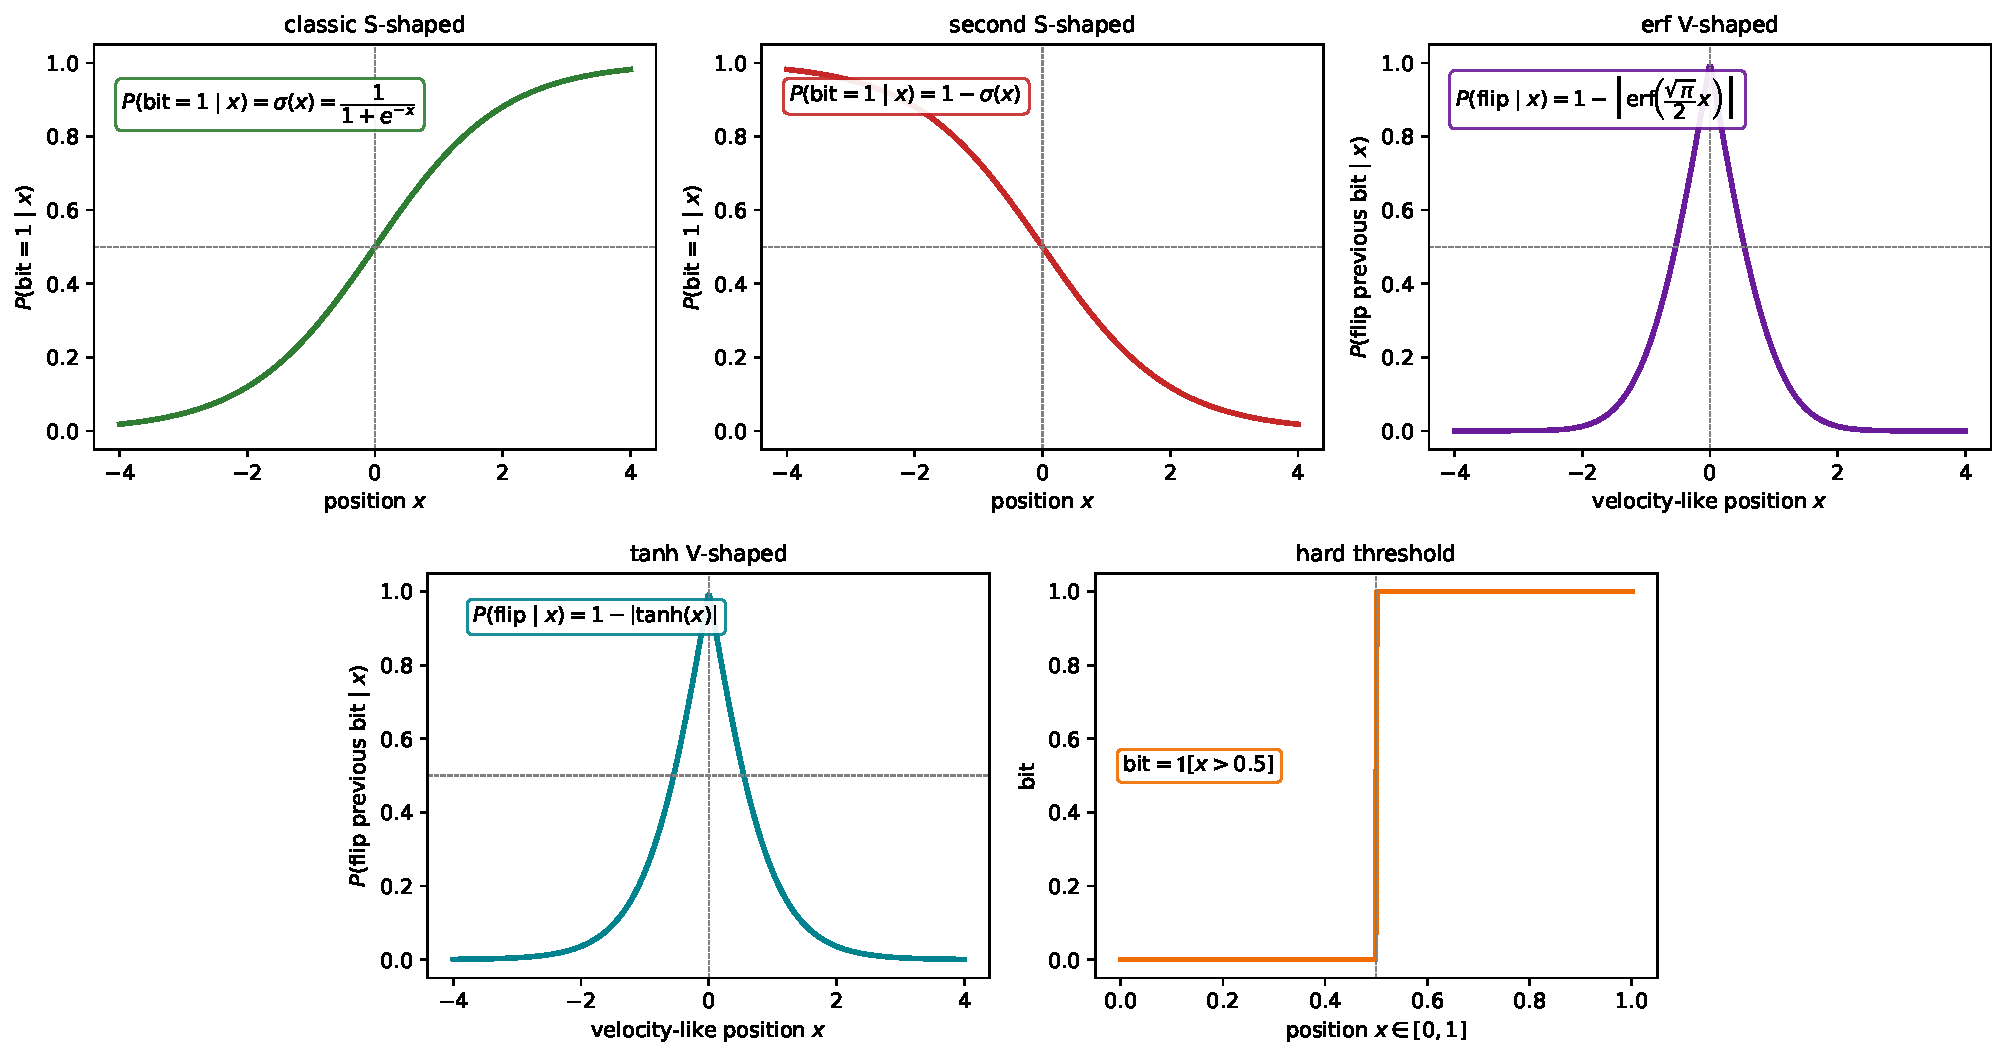
\includegraphics[width=\linewidth]{figures/transfer_functions.pdf}
  \caption{The 5 transfer functions used in this study: 4 are each one
    baseline's own fixed choice, and all 5 together form the proposed
    method's per-particle searched pool (Section~\ref{sec:3.3}). Panel
    titles match the names used throughout this section. Top row, left to
    right: \emph{classic S-shaped} (Eq.~\ref{eq:s-shaped-classic})
    \cite{Kuntalp:2024}; \emph{second S-shaped}
    (Eq.~\ref{eq:s-shaped-baseline}) \cite{Hashemi:2026}; \emph{erf
    V-shaped} (Eq.~\ref{eq:v-shaped}) \cite{Hashemi:2026}. Bottom row,
    centered under the top row: \emph{tanh V-shaped}
    (Eq.~\ref{eq:v-shaped-tanh}) \cite{Mirjalili:2013}; \emph{hard
    threshold} (Eq.~\ref{eq:threshold}) \cite{Hashim:2023}, used natively
    in $[0,1]$ by mHGS/MGWO-eP (the proposed method instead uses the
    rescaled $x>0$ boundary of Eq.~\ref{eq:threshold-rescaled}, not shown
    as a separate panel since it is the same step function shifted).}
  \label{fig:transfer}
\end{figure}





\subsection{Fitness Function}
\label{sec:3.5}

Every candidate solution is scored by a single scalar fitness, combining diagnostic performance with a feature-parsimony penalty in Eq. (\ref{eq:fitness}):
\begin{equation}
  \text{fitness} = \omega \cdot (1 - \text{BalAcc}) + (1 - \omega) \cdot \frac{|S|}{D},
  \label{eq:fitness}
\end{equation}
where $\text{BalAcc}$ is the out-of-fold balanced accuracy (the average of sensitivity and specificity, robust to Oxford's class imbalance \cite{Brodersen:2010}) achieved by the decoded feature subset and ensemble of classifiers, $|S|$ is the number of selected features, $D$ is the total number of available features, and $\omega = 0.9$ weights diagnostic performance nine times as heavily as feature count. This weighted-sum formulation -- a classification-performance term and a feature-cardinality-ratio term combined via a single dominant weight -- follows the same convention used to combine a $k$NN-classifier error rate with a selected-feature ratio in a 2024 whale-optimization-based feature-selection pipeline for Parkinson's disease diagnosis from MRI \cite{Priyadharshini:2024}. This value was chosen so that a modest reduction in feature count is rewarded only when it does not come at a material cost to balanced accuracy, reflecting the clinical framing of this study as favoring parsimonious acoustic measurement panels for low-burden screening, without allowing the parsimony term to dominate the primary diagnostic objective. Lower fitness is better; every optimizer in this study is implemented as a minimizer.

\subsection{The Proposed Method: CSO with a Per-Particle Searched Transfer Function}
\label{sec:3.6}

The proposed method is the original Competitive Swarm Optimizer (CSO)
\cite{Cheng:2015} itself, unmodified -- no additional search strategies are
layered on top of it. Its only departure from a textbook CSO
re-implementation is the encoding it searches over (Section~\ref{sec:3.3}):
each particle carries a transfer-function-selector segment, so which of
5 candidate transfer functions binarizes a given particle is decided by
the search itself, rather than fixed in advance the way every reproduced
baseline fixes its own.

\begin{figure}[t]
  \centering
  
\includegraphics[width=\linewidth]{figures/CSO.pdf}
  \caption{The CSO per-generation flow \cite{Cheng:2015}, unmodified by
    this study: the population is randomly paired into one-on-one
    competitions; each pair's winner passes to the next generation
    unchanged (learning-free), while its loser updates toward the winner
    (learning). Figure~\ref{fig:tf-selector} details what "learning" means
    once the transfer-function-selector segment is part of the loser's
    own position.}
  \label{fig:cso}
\end{figure}

\textbf{Base algorithm (CSO).} The Competitive Swarm Optimizer (CSO)
\cite{Cheng:2015} was originally proposed for \emph{large-scale}
optimization, and departs from the attractor-based update rule common to
PSO and its many derivatives, where every particle is pulled toward one
or two fixed reference points (a personal best, a global best, or
similar) every generation. CSO instead structures each generation as a
set of pairwise competitions: only the loser of each pair updates, and it
draws its next position from whichever particle it happens to be paired
against that generation, rather than from a single swarm-wide attractor
-- a design intended to preserve swarm diversity and scale more
gracefully to high-dimensional search spaces than attractor-based
updates. Concretely, each generation, the population of $N$
particles (an even number) is randomly paired into $N/2$ one-on-one
competitions. Within each pair, the fitter particle (the \emph{winner})
passes to the next generation completely unchanged; the weaker particle
(the \emph{loser}) updates its velocity and position toward the winner:
\begin{align}
  v_l &\leftarrow r_1 v_l + r_2 (x_w - x_l) + \phi \, r_3 (\bar{x} - x_l), \\
  x_l &\leftarrow x_l + v_l,
\end{align}
where $x_w, x_l$ are the winner's and loser's positions, $\bar{x}$ is the
population mean position, $r_1, r_2, r_3$ are independent uniform random
vectors, and $\phi$ is CSO's social-term control coefficient (Eq.\ 25--26,
\cite{Cheng:2015}), which is exactly 0 for the swarm sizes used in this
study ($N=30 \le 100$) -- so plain CSO at this scale has no mean-position
pull at all, only the winner-attraction and inertia terms.

\textbf{Per-particle transfer-function selection.} Every loser's update
above operates on its \emph{entire} position, including the
transfer-function-selector segment introduced in Section~\ref{sec:3.3} --
so a loser's selector segment is updated by the same velocity/position
rule as the rest of its position, and can therefore change which
transfer function that particle uses from one generation to the next.
Once a loser's new position is computed, it is decoded in two steps
(Figure~\ref{fig:tf-selector}): first, an argmax over its own leading
5-dim selector segment picks one of the 5 candidate transfer functions of
Section~\ref{sec:3.4}; second, that candidate binarizes the particle's
trailing $D+5$ dimensions into the feature mask and classifier mask used
to evaluate its fitness. Winners are unaffected, since they are carried
over completely unchanged, selector segment included.

\begin{figure}[t]
  \centering
  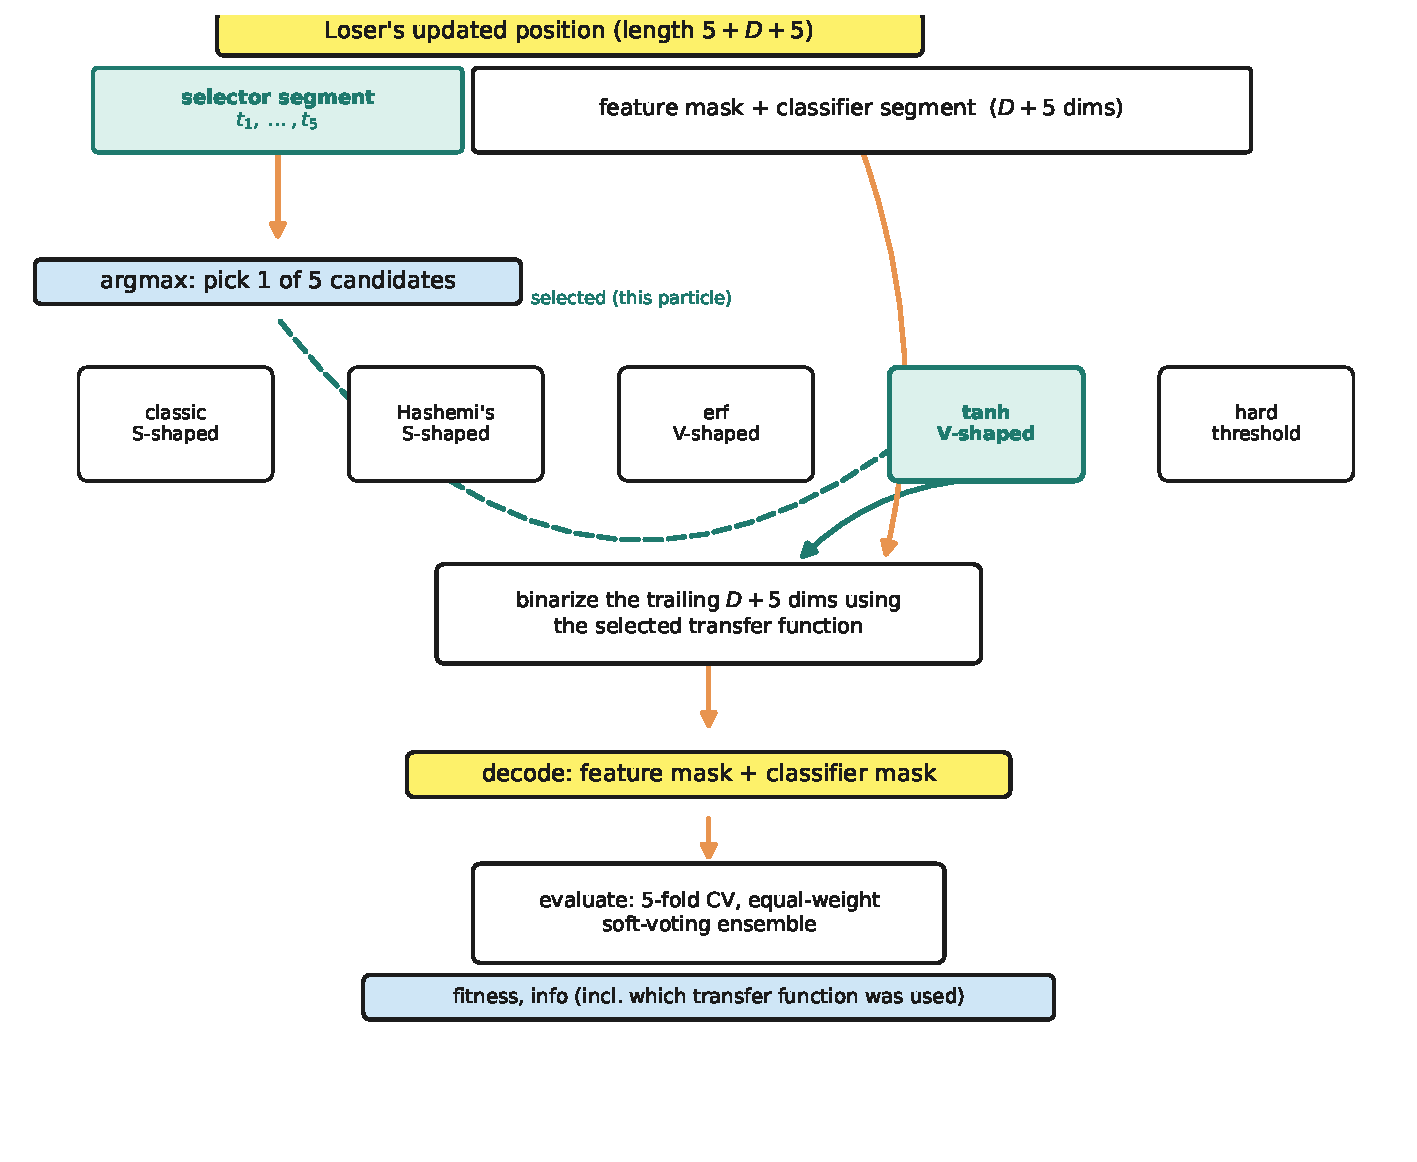
\includegraphics[width=\linewidth]{figures/cso_tf_selector_diagram.pdf}
  \caption{Decoding a loser's updated position once the
    transfer-function-selector segment is part of it. The leading 5-dim
    segment $t_1,\dots,t_5$ is argmaxed to pick one of the 5 candidate
    transfer functions (Section~\ref{sec:3.4}); the chosen candidate then
    binarizes the trailing $D+5$ dimensions into a feature mask and
    classifier mask, which are evaluated exactly as in
    Figure~\ref{fig:encoding}. Different particles, and the same particle
    across generations, may resolve to different candidates.}
  \label{fig:tf-selector}
\end{figure}

\subsection{Comparison Methods}
\label{sec:3.7}

\textbf{Reproduced literature baselines.} Seven metaheuristic
feature-selection methods from five recent source papers are
re-implemented from their published equations and evaluated under this
study's own encoding, fitness function, and cross-validation protocol
(not each source paper's own classifier or data split), enabling a
controlled, like-for-like comparison against the proposed method: BPSO and BBOA
(binary particle swarm and butterfly optimization, hybrid S-shaped/
V-shaped transfer function) \cite{Hashemi:2026}; BGWO and HybridGWO
(binary grey wolf optimizer, and a whale-optimization-then-grey-wolf
refinement cascade) \cite{AlNajjar:2024}; MGWO-eP (grey wolf optimizer
with an exponentially-decaying exploration coefficient)
\cite{Santhosh:2025}; mHGS (modified Hunger Games Search with a
mean-of-best-4 local escaping operator) \cite{Hashim:2023}; and QMFO
(Mayfly Algorithm with a quantum-rotation-gate mutation operator)
\cite{Mansour:2024}. A third variant originally reproduced from Hashemi
et al. \cite{Hashemi:2026}, BWOA (binary whale optimization), was also
implemented but is excluded from the reported comparison: of the 8
originally reproduced baselines, its results were consistently the
weakest and least consistent with its own source paper's claims, so it is
not included as a fair comparison point (see Section~\ref{sec:5.4} for
further discussion). Where a source paper does not fully specify an
equation
(most application papers cite only the base metaheuristic by name), the
canonical published form of that equation is used instead, and every such
gap-fill is documented in the corresponding source file's docstring for
transparency.

\textbf{Equal evaluation budget.} Every optimizer -- the proposed method and
baselines alike -- is compared under an equal fitness-evaluation budget
(\texttt{max\_evaluations}), not equal generation count, since different
algorithms spend different numbers of fitness evaluations per generation
(e.g., the hybrid S-shaped/V-shaped transfer function used by
BPSO/BBOA evaluates two binarization candidates per individual per
generation; mHGS's production and escaping operators each conditionally
add extra evaluations). A population size of 30 and an evaluation budget
of 3000 fitness evaluations per run are used throughout; each algorithm's
internal time-dependent schedule (e.g. the grey
wolf family's exploration coefficient) is normalized against a
\emph{nominal} generation count derived from this budget, while the
budget itself remains the sole stopping condition.

\textbf{Independent runs and seeding.} Each algorithm-dataset combination
is run for multiple independent seeds (seed $= 2026 + 50 \times$
run index, so seeds do not overlap across runs), with all stochastic
elements -- population initialization, transfer-function sampling, and
the cross-validation fold assignment for that seed -- freshly drawn each
run. The head-to-head comparison against the 7 baselines uses a number of
runs sufficient to support the statistical testing described in
Section~\ref{sec:3.9}.

\subsection{Evaluation Metrics}
\label{sec:3.8}

For every run, the out-of-fold predictions used to compute fitness
(Section~\ref{sec:3.5}) are also used to report a full panel
of standard diagnostic-performance metrics, computed once per run (not
re-derived from the fitness value): accuracy, balanced accuracy,
\textbf{sensitivity (recall)}, \textbf{specificity}, precision, F1-score,
and area under the receiver operating characteristic curve (ROC-AUC).
Sensitivity and specificity are reported alongside the more
ML-conventional accuracy/F1/AUC metrics because they are the standard
vocabulary for evaluating a clinical screening tool: sensitivity
quantifies the fraction of true PD cases the pipeline would flag (missed
cases have direct clinical cost), while specificity quantifies the
fraction of healthy individuals correctly spared unnecessary follow-up.
Feature-selection ratio ($|S|/D$) and the identity of the selected
feature subset and active classifier(s) are also recorded for every run,
supporting the feature-interpretability analysis in
Section~\ref{sec:5.5} and the classifier-preference analysis in
Section~\ref{sec:5.6}.

\subsection{Statistical Analysis}
\label{sec:3.9}

Because every algorithm is run under the same set of seeds (and therefore
the same sequence of cross-validation fold assignments per run index),
per-run performance scores across algorithms are paired rather than
independent samples. The Wilcoxon signed-rank test \cite{Wilcoxon:1945} is
used for pairwise comparisons between the proposed method and each
individual baseline, and the Friedman test \cite{Friedman:1937} is used
to test for an overall difference across the full set of compared
algorithms before conducting pairwise follow-up tests, guarding against
inflated false-positive rates from running many uncorrected pairwise
tests -- following established recommendations for comparing multiple
classifiers across multiple datasets \cite{Demsar:2006}
(\texttt{src/experiments/stats.py}).

\subsection{Implementation Details}
\label{sec:3.10}

All optimizers, the fitness evaluator, and the experiment orchestration
are implemented in Python (NumPy for optimizer internals; scikit-learn
\cite{Pedregosa:2011} and XGBoost \cite{Chen:2016} for the candidate
classifiers). Runs are executed serially
(one fitness evaluation, and one classifier fit, at a time) on
consumer-grade hardware; each completed run is checkpointed to disk
immediately so that a long-running batch of independent runs can be
resumed from the last completed run rather than restarted from scratch
after an interruption.
